\chapter{Introduction}
\section{eBusiness Information et Excilys}

\subsection{La Charte Excilys}
eBusiness Information a été créée en l'an 2000 dans le but de répondre à des problématiques métier diverses grâce à la mise en place de solutions informatiques robustes, tout en mettant en valeur de savoir-faire humain qui amène à ces solutions.

En effet, pour ses fondateurs, le service informatique est un métier d'hommes qui doivent avoir de plus en plus de compétences. En 2002, ils imaginent une notion nouvelle dans le monde du service informatique : le \em{Service équitable}. Inspiré par le commerce équitable, cette notion sera inscrite dans une charte : la \em{Charte Excilys}. Le service équitable consiste en la création d'un cercle vertueux\footnote{L'entreprise facture le client plus cher que la moyenne. Cette facturation profite au consultant qui fournit donc un travail de qualité. Ce travail de qualité satisfait le client. Ainsi, les acteurs concernés par le service rendu y trouvent tous leur compte.} profitant à tous les acteurs du service. Tout comme le commerce équitable, cette notion vise à profiter aux personnes qui produisent le service plutôt qu'aux intermédiaires seuls.

La \em{Charte Excilys} définit donc un ensemble de droits et de devoirs entre les trois acteurs du service : le client, l'entreprise et le consultant comme montré figure \ref{droits_devoirs}.

\begin{figure}[h]
\begin{center}
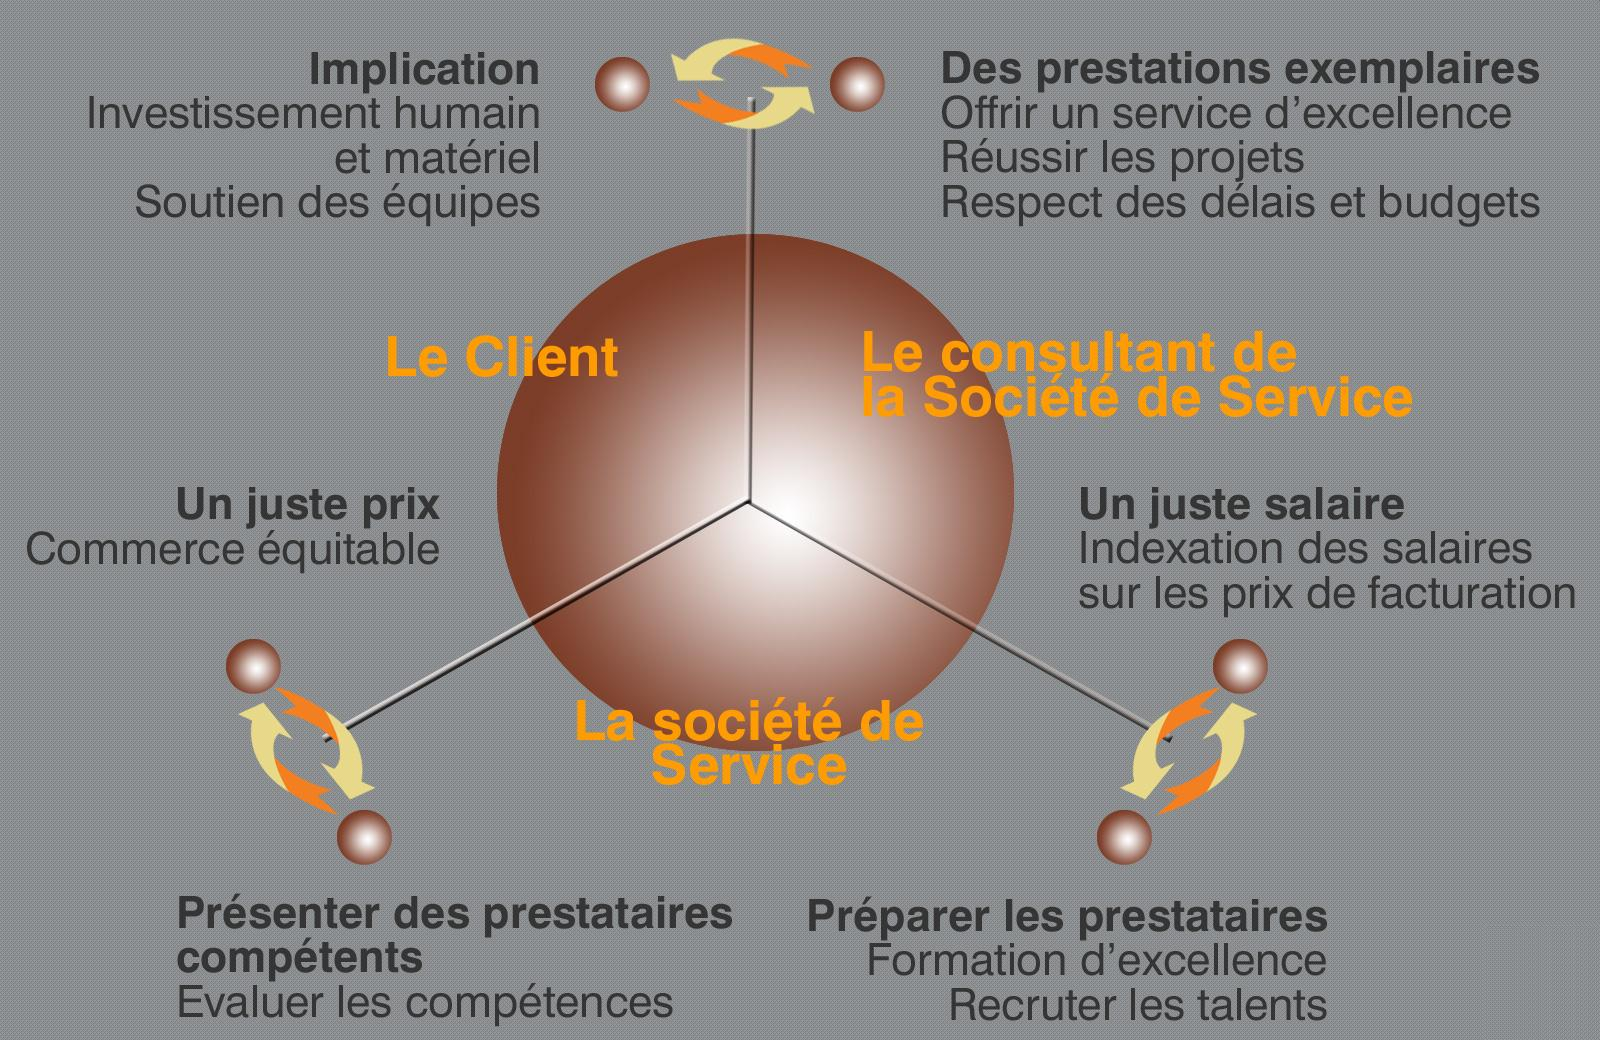
\includegraphics[width=200pt]{img/droits_devoirs.jpg}
\end{center}
\caption{Droits et devoirs pour les acteurs du service équitable}
\label{droits_devoirs}
\end{figure}

L'application des règles de cette charte était un pari risqué, mais un pari réussi. En effet, après plusieurs années de fonctionnement, eBusiness Information a prouvé qu'un modèle basé sur les compétencespeut fonctionner. De plus, les résultats de l'entreprise sont extrêmement encourageants : relations durables avec les clients, aucunes dettes, aucun investisseur extérieur et aucun projet raté.

\subsection{Le groupe Excilys}

Le groupe Excilys est né de la volonté de reproduire ce modèle dans d'autres sociétés de service qui souhaitent aussi centrer leur métier sur l'excellence dans leur métier ; c'est d'ailleurs du mot excellence que vient le nom \em{Excilys}.

Depuis, plusieurs entreprises ont rejoint le groupe, elles sont aujourd'hui au nombre de sept : Adlys, Altendis, eBusiness Information, Edvance, Equitalis, SS2J et Visual3X. Chacune de ces sociétés fournit des services en informatique mais avec des domaines de compétence complémentaires et une image de qualité qui lui est propre.
  
\section{Formation Java/JEE}

\subsection{Le stagiaire chez eBusiness Information}

Excilys\footnote{Dans le reste de ce rapport, eBusiness Information et Excilys, bien que représentant deux entités juridiques différentes, désigneront l'entreprise où j'ai réalisé mon stage.} emploie beaucoup de stagiaires chaque année ; par exemple, pour l'année 2011, c'est plus d'une vingtaine de stagiaires qui a réalisé son stage chez Excilys. L'entreprise mise beaucoup sur les jeunes informaticiens qui sortent de l'école afin d'embaucher des consultants compétents qui lui permettront de continuer à offrir un service  de qualité à ses clients.

Dans cette optique, un grand soin est apporté au confort des stagiaires : hébergement disponible, salaire intéressant, et, surtout, une formation de six semaines au début du stage afin de lui permettre de monter en compétence sur de nombreuses technologies. Le fait que les stagiaires soient en colocation dans le même immeuble, et qu'ils travaillent dans le même open space permet de créer rapidement des liens et cela participe à une émulation générale, ainsi qu'à une bonne ambiance.

A la suite de la formation, chaque stagiaire se voit proposer un sujet de stage différent, et, parfois, une mission chez un client jusqu'à la fin de son stage, et après. 

\subsection{Capico}

Afin de former ses stagiaires, et d'offrir à ses consultants la possibilité de se former facilement sur diverses technologies utilisées dans le domaine Java/JEE, les gérants d'eBusiness Information ont investi dans le développement d'un outil de formation en ligne nommé \em{Capico}. Cet outil contient des cours (audio ou non) ainsi que des exercices et tp avec leur corrigé, la figure \ref{capico} représente l'interface de Capico.

\begin{figure}[ht]
\begin{center}
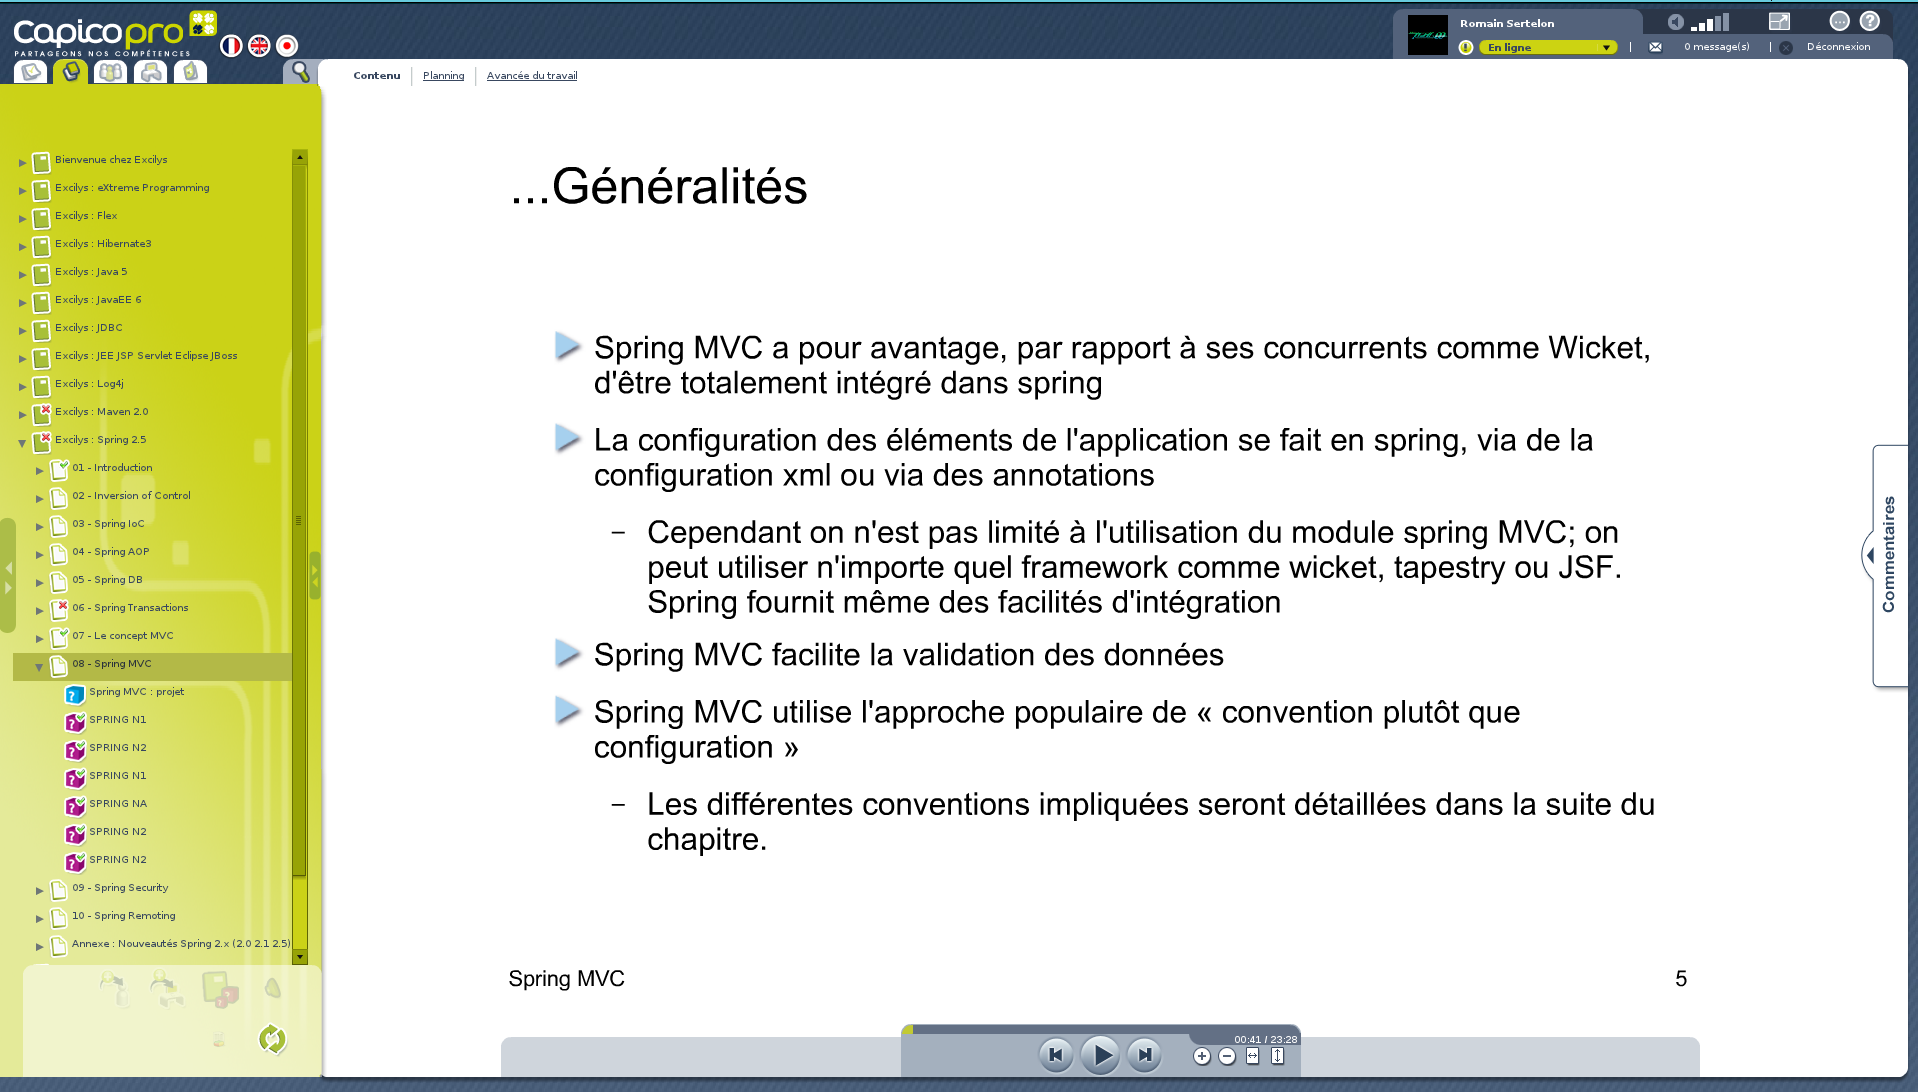
\includegraphics[width=400pt]{img/capico.png}
\end{center}
\caption{Interface de Capico}
\label{capico}
\end{figure}

Aujourd'hui, Capico\footnote{Capico pour \em{Capi}talisation des \em{co}nnaissances} est bien plus qu'un outil de formation interne. En effet, avec le temps, et grâce aux investissements en R\&D d'Excilys, ce logiciel est devenu une plateforme d'e-coaching qui propose des cours gratuits du CP au CM2, en français et mathématiques et qui est récemment entré en compétition dans un appel d'offre du département des Hauts-de-Seine afin de moderniser ses collèges.  

\subsection{Contenu de la formation}

\subsubsection{Cours sur Capico}
La période de six semaines de formation commence par des cours sur Capico couvrant diverses technologies mais aussi des notions sur les méthodes agiles, en particulier \em{eXtreme Programming}. Les technologies abordées sont les suivantes :

\begin{itemize}
  \item \em{UML / Java 5} - Un rappel sur Java et le langage de formalisation UML ;
  \item \em{JEE JSP+Servlets / Java EE 6} - Un rappel sur Java Enterprise (EJB, Servlet, JSP, JSF) ;
  \item \em{JDBC / Hibernate} - Un cours sur JDBC et Hibernate, l'ORM Java le plus répandu ;
  \item \em{Log4j / Slf4j} - Un cours sur la journalisation en Java ;
  \item \em{JUnit} - Un cours sur le framework JUnit qui permet de faire du test unitaire ;
  \item \em{Spring} - Un cours sur le framework Spring (IoC, MVC, etc.) beaucoup utilisé en entreprise ;
  \item \em{Maven} - Un cours sur un gestionnaire de dépendances de plus en plus utilisé au sein de la communauté Java ;
  \item \em{Subversion / Git} - Un cours sur les deux gestionnaires de sources ;
  \item \em{Flex} - Un cours expliquant les bases du développement avec Flex.
\end{itemize}

Un tour d'horizon des technologies les plus utilisées par les clients de l'entreprise, ainsi que les technologies utilisées au sein du projet Capico, chaque stagiaire passant sur ce projet avant d'être affecté à une mission ou à un projet différent.

\subsubsection{Réalisation d'un projet}

La formation, est complétée par la mise en pratique des cours grâce à la réalisation d'une application d'ebanking dans des conditions agiles. Notre groupe de six stagiaires à réalisé son application\footnote{Disponible sur Github : http://github.com/BluePyth/patricks-bank} sur cinq semaines, soit cinq itérations en programmant en binômes tel que préconisé par la méthode eXtreme Programming. La figure \ref{patricks_bank} représente le site que nous avons réalisé.

\begin{figure}[h]
\begin{center}
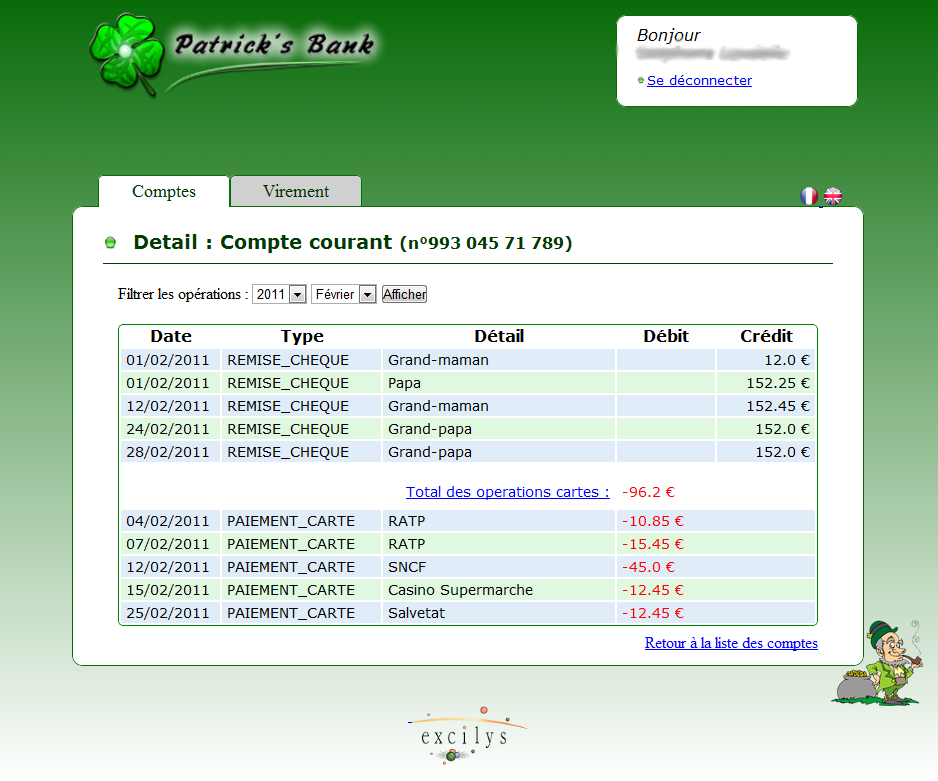
\includegraphics[width=400pt]{img/patricks_bank.png}
\end{center}
\caption{Patrick's Bank - Visualisation du détail d'un compte}
\label{patricks_bank}
\end{figure}

Nous avons pu ainsi nous confronter aux technologies que nous n'avions jusqu'alors pas pratiquées : Intégration Continue avec Jenkins, utilisation de Google code, de Maven, etc. 

\section{Ma mission}
A la fin de la période de formation, j'ai commencé à travailler sur Capico, comme tous les autres stagiaires, puis Stéphane Landelle m'a proposé de travailler avec lui sur une idée dont il avait réalisé une \em{Preuve de Concept}. Cette idée concerne la création d'un nouvel outil de test de montée en charge - ou injecteur HTTP - nommé Gatling.

Dès lors, ma mission a été de travailler sur ce nouveau projet, le concevoir, puis implémenter les fonctionnalités que l'outil doit proposer. L'objet de ce rapport est donc de présenter la manière dont j'ai réalisé cet outil.

Chap X présente ceci, etc.